\chapter{PICKING E MODELAGEM DIRETA}
\label{cap2}

Após a obtenção da seção empilhada utilizando o empilhamento CRE \cite{relatorio}, realizamos o picking dos tempos de trânsito sobre os refletores na seção. Estes tempos de trânsito são tempos duplos de reflexão para cada par t0 m0.

\begin{figure}[H]
\caption{Geometria do arranjo ERC.}
\begin{center}
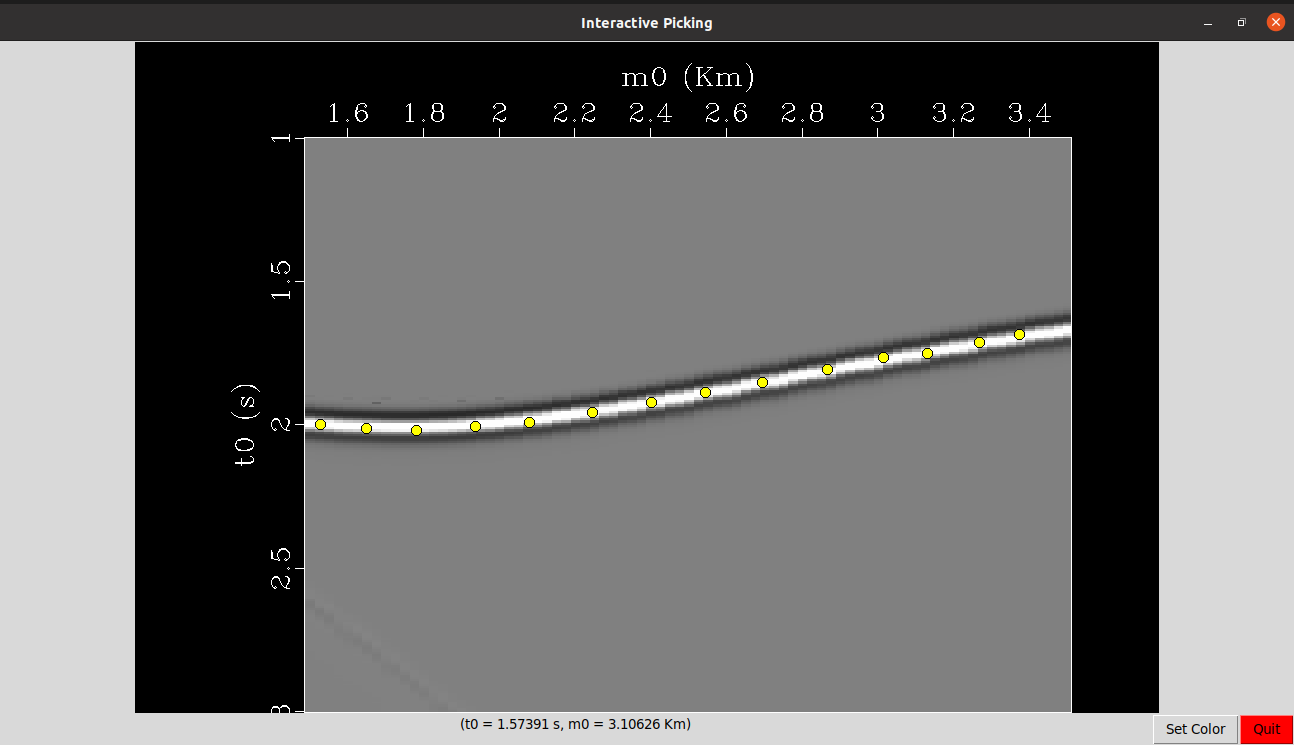
\includegraphics[scale=0.3]{images/picking.png}
\vspace{-0.3cm}
\end{center}
\begin{center}
 Fonte: Do Autor.
\end{center}
\label{fig:2.1}
\end{figure}

Estes tempos de trânsito são utilizados para traçar raios da superfície de aquisição em direção ao modelo
até que o tempo de trânsito seja consumido
o modelo inicial é um modelo de velocidades constante

cada raio é iniciado na superfície de aquisição na posição da coordenada m0 e é lançado com a direção dada
pelo parâmetro BETA0. O final do raio é o ponto inicial NIP localização. O vetor vagarosidade no ponto é
Normal ao refletor, e com estas informações, o modelo inicial é configurado \cite{niptomo}

\begin{figure}[H]
\caption{Geometria do arranjo ERC.}
\begin{center}
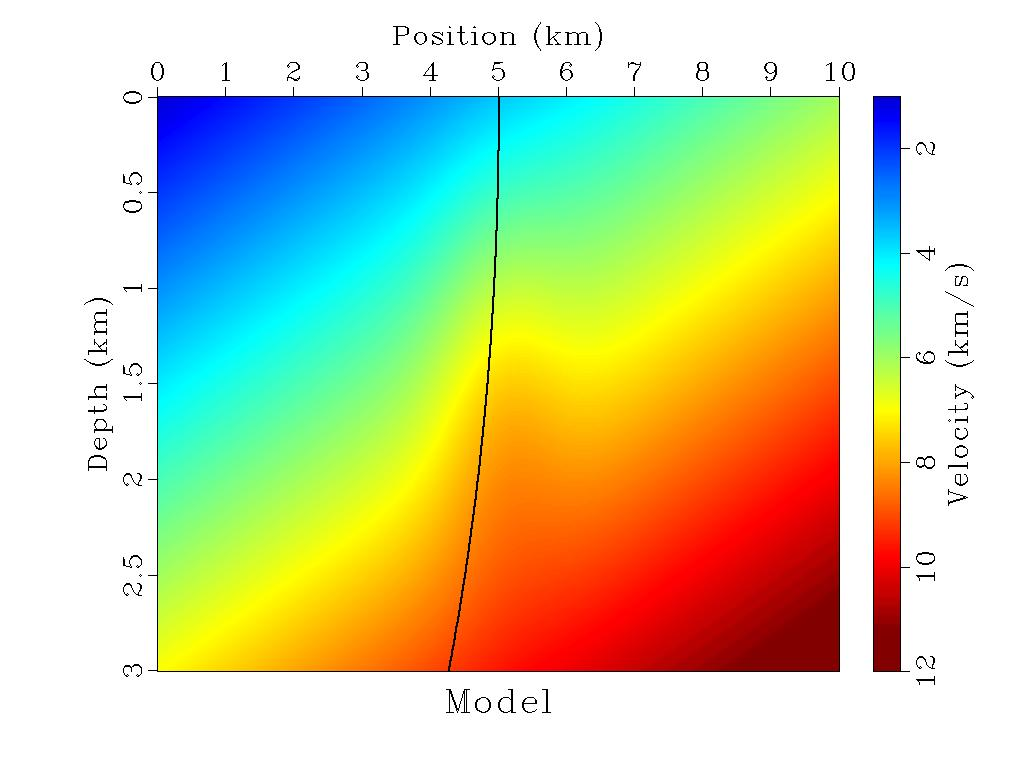
\includegraphics[scale=0.3]{images/raiomodelo.jpg}
\vspace{-0.3cm}
\end{center}
\begin{center}
 Fonte: Do Autor.
\end{center}
\label{fig:2.2}
\end{figure}

Iniciando da posição da fonte NIP determinada anteriormente, um leque de raios é lançado em direção 
a superfície de aquisição e os tempos de trânsito são armazenados e somados \cite{stereo}

\begin{figure}[H]
\caption{Geometria do arranjo ERC.}
\begin{center}
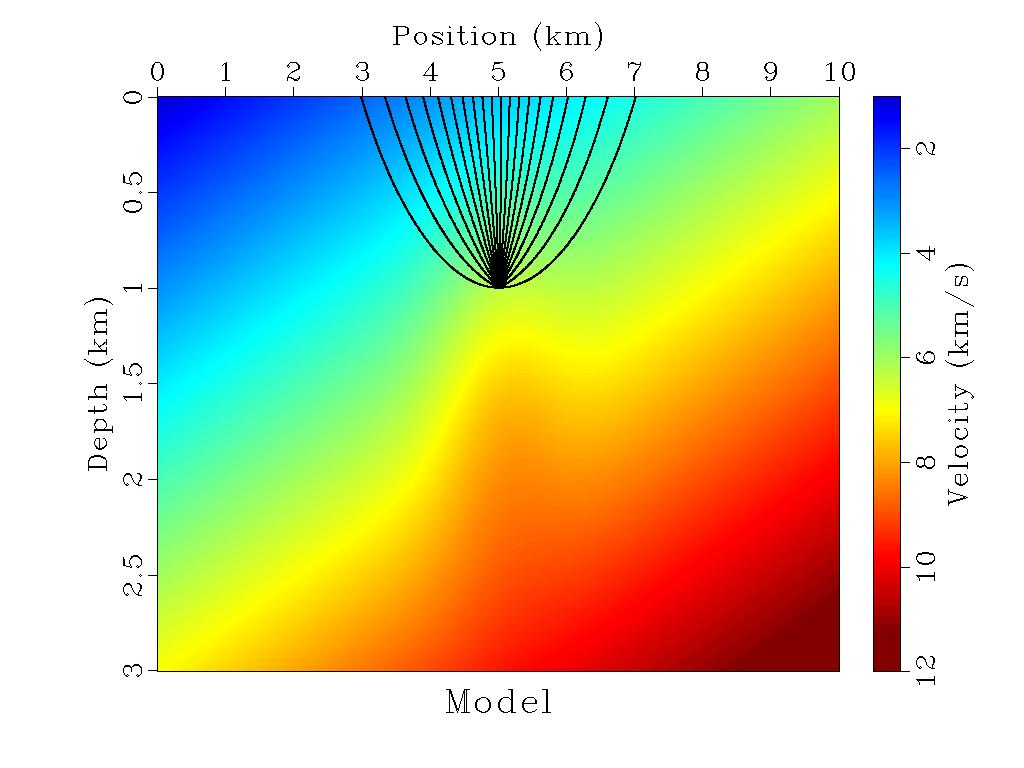
\includegraphics[scale=0.3]{images/raioleque.jpg}
\vspace{-0.3cm}
\end{center}
\begin{center}
 Fonte: Do Autor.
\end{center}
\label{fig:2.3}
\end{figure}



